\documentclass[10pt,landscape]{article}
\usepackage[utf8]{inputenc}
\usepackage{multicol}
\usepackage{calc}
\usepackage{ifthen}
\usepackage[landscape]{geometry}
\usepackage{hyperref}
\usepackage{amsmath}
\usepackage{amssymb}
\usepackage{tabularx}
\usepackage{caption}
\usepackage{verbatim}
\usepackage{systeme}
\usepackage{nicefrac}
\usepackage{accents}
\usepackage{enumitem}
\usepackage[printwatermark]{xwatermark}
\usepackage{tikz}
\usetikzlibrary{calc,matrix}
\usepackage[compact]{titlesec}
\usepackage{microtype}
\usepackage[flushleft]{threeparttable}
\usepackage{textcomp}
\usepackage{pifont}

% This sets page margins to .5 inch if using letter paper, and to 1cm
% if using A4 paper. (This probably isn't strictly necessary.)
% If using another size paper, use default 1cm margins.
\ifthenelse{\lengthtest { \paperwidth = 11in}}
{ \geometry{top=.5in,left=.5in,right=.5in,bottom=.5in} }
{\ifthenelse{ \lengthtest{ \paperwidth = 297mm}}
	{\geometry{top=1cm,left=1cm,right=1cm,bottom=1cm} }
	{\geometry{top=1cm,left=1cm,right=1cm,bottom=1cm} }
}

% Turn off header and footer
\pagestyle{empty}

% Reduce size of \section e \subsection
\titleformat{\section}{\normalfont\large\bfseries}{\thesection}{1em}{}
\titleformat{\subsection}{\normalfont\normalsize\bfseries}{\thesubsection}{1em}{}
\titlespacing{\section}{0pt}{0ex}{-0.5ex}
\titlespacing{\subsection}{0pt}{0ex}{-0.5ex}

% Define BibTeX command
\def\BibTeX{{\rm B\kern-.05em{\sc i\kern-.025em b}\kern-.08em
		T\kern-.1667em\lower.7ex\hbox{E}\kern-.125emX}}

% Don't print section numbers
\setcounter{secnumdepth}{0}


\setlength{\parindent}{0pt}
\setlength{\parskip}{0pt plus 0.5ex}

% <v,w> prodotto scalare
\newcommand{\product}[2]{\langle\,#1,#2\,\rangle}
% sottolinea i vettori
\renewcommand{\vec}[1]{\underline{#1}}
% funzioni non defininte
\newcommand{\tr}{\mathrm{tr}}
\newcommand{\diag}{\mathrm{diag}}
\newcommand{\rk}{\mathrm{rk}}
\newcommand{\sgn}{\mathrm{sgn}}
\newcommand{\Col}{\mathrm{Col}}
\newcommand{\Row}{\mathrm{Row}}
\newcommand{\Imm}{\mathrm{Im}}

\setlist[itemize]{noitemsep, nolistsep}

% numeri cerchiati
\newcommand*\circled[1]{\tikz[baseline=(char.base)]{
		\node[shape=circle,draw,inner sep=2pt] (char) {#1};}}

\newcommand{\Lin}{\mathcal{L}}
\newcommand{\Base}{\mathcal{B}}
\newcommand{\Case}{\mathcal{C}}

\newcommand{\cmark}{\ding{51}}%
\newcommand{\xmark}{\ding{55}}%

%\newwatermark[allpages,color=black!10,angle=45,scale=6,xpos=-20,ypos=15]{BOZZA}

\begin{document}

\raggedright
\footnotesize
\begin{multicols}{3}

% multicol parameters
% These lengths are set only within the two main columns
%\setlength{\columnseprule}{0.25pt}
\setlength{\premulticols}{1pt}
\setlength{\postmulticols}{1pt}
\setlength{\multicolsep}{1pt}
\setlength{\columnsep}{2pt}

{\Large{\textbf{Geometria e Algebra Lineare II}}}

\section{Autovalori e autovettori}

$V$ spazio vettoriale su $K$ di dimensione $n$, $f: V \rightarrow V$, \vec{v} è autovettore associato all'autovalore $\lambda$:
\begin{tabular}{ll}
	$\vec{v} \ne \vec{0}$ & $f(\vec{v}) = \lambda \vec{v}$ \\
	$k\vec{v}$ & autovettore associato a $\lambda$
\end{tabular}

Per trovare gli autovalori risolvere $\det(A-\lambda I) = 0$. Il determinante viene chiamato \emph{polinomio caratteristico} ($p(\lambda)$).
L'autospazio di $\lambda$ è $V_\lambda = \ker(A-\lambda I)$

\begin{tabular}{ll}
	molt. algebrica ($m_a$) & moltiplicità di $\lambda$ in $p(\lambda)$ \\
	molt. geometrica ($m_g$) & dimensione di $V_\lambda$
\end{tabular}

\begin{tabular}{l}
	$\lambda_1 \ne \lambda_2 \implies V_{\lambda_1} \cap V_{\lambda_2} = \{\vec{0}\}$ \\
	$\det(A-\lambda I) = (-1)^n (\lambda - \lambda_1) (\lambda - \lambda_2) \cdots (\lambda - \lambda_n)$ \\
	$\det A = \lambda_1 \lambda_2 \cdots \lambda_n$ \\
	$\tr A = \lambda_1 + \lambda_2 + \cdots + \lambda_n$ \\
	$\lambda_i \ne \lambda_j \quad \vec{v}_i \in V_{\lambda_i} \quad \vec{v}_j \in V_{\lambda_j} \implies \vec{v}_i$ l.i. $\vec{v}_j$ \\
	$1 \le m_g \lambda \le m_a \lambda$ \\
	$\lambda$ è regolare sse $m_a \lambda = m_g \lambda$ \\
	$\lambda \text{ autoval di } A \implies \lambda^k \text{ autoval di } A^k \quad (k > 0)$ \\
	$\lambda \text{ autoval di } A \implies 1/\lambda \text{ autoval di } A^{-1}$ \\
	$\sgn A = (t,r,s)$ (segnatura, numero autoval +/-/0)
\end{tabular}
\section{Matrici simili}

A e B sono matrici simili se esiste P t.c. $A = P^{-1}BP$. Condizioni necessarie (e sufficienti se $n \le 3$) per A simile B:

\begin{tabular}{l}
	Stesso polinomio caratteristico \\
	Stessi autoval (e risp. molt.), autovett, det. e traccia \\
	Stesso rango
\end{tabular}

A è diagonalizzabile se è simile ad una matrice diagonale. A è diagonaliz. sse ammette $n$ autovett. linearmente indipendenti. $P^{-1}AP = \diag(\lambda_1, \lambda_2, \dots, \lambda_n)$. $P=[ \vec{c}_1 | \cdots | \vec{c}_n ]$ $\vec{c}_i \in V_{\lambda_i}$ e $\vec{c}_i$ linearmente indipendente da $\vec{c}_j$.

Se A ha $n$ autoval. distinti allora è diagonaliz. (non necess.). A è diagonaliz. sse tutti i suoi autoval. sono regoalri

\section{Verificare se A è diagonalizzabile}
\begin{enumerate}[noitemsep]
	\item Calcolare gli $n$ autoval. di A. Se non sono tutti reali \xmark
	\item Calcolare le $m_a$ degli autoval. Se sono tutte 1 \cmark
	\item Verificare che $m_a \lambda > 1 \Rightarrow m_a \lambda = m_g \lambda$ \cmark
\end{enumerate}

\section{Verificare se A e B sono simili}
\begin{enumerate}[noitemsep]
	\item Traccia, determinante o rango diversi \Frowny{}
	\item $\det(A-\lambda I) \ne \det(B-\lambda I)$ \Frowny{}
	\item $\exists \lambda_i: m_{g_A} \lambda_i \ne m_{g_B} \lambda_i$ \Frowny{}
	\item $n \le 3$ \Smiley{}
	\item A e B entrambe diagonaliz. \Smiley{}
	\item Solo una tra A e B è diagonaliz. \Frowny{}
	\item XA = BX e $\det X \ne 0$ \Smiley{} altrimenti \Frowny
\end{enumerate}

\section{Teorema di Hamilton-Cayley}

Se $p(\lambda)$ è polinomio caratteristico di $A$ allora $p(A) = 0$. Esempio: $p(\lambda) = 5\lambda^2-5\lambda-2$ allora $5A^2-5A-2=0$

\section{Spazi euclidei}

Uno spazio euclideo è uno spazio vettoriale su R dotato di prodotto scalare.

\begin{tabular}{ll}
	Norma & $||\vec{v}|| = \sqrt{\product{\vec{v}}{\vec{v}}}$ \\
	Versore & $||\vec{u}|| = 1$ \\
	Ortogonalità & $\vec{u} \perp \vec{v} \iff \product{\vec{u}}{\vec{v}} = 0$ \\
	Carnot & $||\vec{u}+\vec{v}||^2 = ||\vec{u}||^2+||\vec{v}||^2+2\product{\vec{u}}{\vec{v}}$ \\
	Pitagora & $\vec{u} \perp \vec{v} \iff ||\vec{u}+\vec{v}||^2 = ||\vec{u}||^2+||\vec{v}||^2$ \\
	Distanza & $||\vec{u}-\vec{v}||$ \\
	Proiezione $\vec{v}$ su $\vec{b}$ & $\vec{v}' = \frac{\product{\vec{v}}{\vec{b}}}{||\vec{b}||^2}\vec{b}$ (coefficiente di Fourier) \\
	Angolo & $\cos \theta = \frac{\product{\vec{u}}{\vec{v}}}{||\vec{u}||\,||\vec{v}||}$ \\
	Dis. triangolare & $||\vec{u}+\vec{v}|| \le ||\vec{u}||+||\vec{v}||$ \\
	Dist. punto-piano & $\frac{|ax_0 + by_0 + cz_0 + d|}{\sqrt{a^2 + b^2 + c^2}}$ \\
	Dist. punto-retta & $||\vec{u} \times \overline{P_0Q}||$ ($\vec{u}$ versore di $r$, $Q \in r$) \\
	Dist. retta-retta & $\frac{|\product{\overline{P_1P_2}}{\vec{r_1} \times \vec{r_2}}|}{||\vec{r_1} \times \vec{r_2}||}$ ($P_1 \in r_1$, $P_2 \in r_2$)
\end{tabular}

Norma: $f: V \rightarrow \mathbb{R}$ t.c.
\begin{tabular}{lll}
	$||t\vec{v}|| = |t|\,||\vec{v}||$ &
	$||\vec{v}|| = 0$ sse $\vec{v} = \vec{0}$ &
	$||\vec{u}+\vec{v}|| \le ||\vec{u}||+||\vec{v}||$
\end{tabular}

Base ortonormale: $\Base = \{\vec{q}_1, \vec{q}_2, \dots, \vec{q}_n\}$ dove $\delta_{ij} = \product{\vec{q}_i}{\vec{q}_j}$ con $\delta_{ij} = 0$ quando $i \ne j$ e $\delta_{ij} = 1$ quando $i = j$

$U = [\vec{q}_1 | \cdots | \vec{q}_n] \iff U^TU=I_n$

\section{Matrici ortogonali}

U è ortogonale se è reale e $U^TU=I_n$:

\begin{tabular}{lll}
	$\det U = \pm1$ & $U^{-1}=U^T$ & $\lambda = \pm 1$
\end{tabular}

$f$ rappresentata da $U$ orto. è un'isometria (conserva la norma).

\begin{tabular}{lll}
	In $\mathbb{R}^2$ &
	$
		M_1 = \begin{bmatrix}
			\cos\theta & -\sin\theta \\
			\sin\theta & \cos\theta \\
		\end{bmatrix}
	$ &
	$
		M_2 = \begin{bmatrix}
			\cos\theta & \sin\theta \\
			\sin\theta & -\cos\theta \\
		\end{bmatrix}
	$
\end{tabular}

$M_1$ ($\det = 1$) rappresenta una rotazione del piano di $\theta$. $M_2$ ($\det = -1$) rappresenta una simmetria rispetto $V_1 = \Lin(\cos\frac{\theta}{2}, \sin\frac{\theta}{2})$.

\section{Algoritmo di Gram-Schmidt}

Sia V uno spazio euclideo e $\vec{v}_1, \vec{v}_2, \dots, \vec{v}_n$ l.i. in V:
\begin{itemize}
	\item $\vec{b}_1 = \vec{v}_1$
	\item $\vec{b}_2 = \vec{v}_2 - \frac{\product{\vec{v}_2}{\vec{b}_1}}{||\vec{b}_1||^2}\vec{b}_1$
	\item $\vec{b}_h = \vec{v}_h - \left(
		\frac{\product{\vec{v}_h}{\vec{b}_1}}{||\vec{b}_1||^2}\vec{b}_1 +
		\cdots +
		\frac{\product{\vec{v}_h}{\vec{b}_{h-1}}}{||\vec{b}_{h-1}||^2}\vec{b}_{h-1}
	\right)$
\end{itemize}

$\Base = \{\vec{b}_1, \vec{b}_2, \dots, \vec{b}_n\}$ è una \textbf{base ortogonale} di $V$.

\section{Proiezioni ortogonali}

Sia H un sottospazio di V:

$H^\perp = \{\vec{v}\text{ ortogonale ad H}\}$ sottospazio di V

\begin{tabular}{lll}
	$(H^\perp)^\perp = H$ & $H\cap H^\perp = \{\vec{0}\}$ & $V=H\oplus H^\perp$
\end{tabular}

$f: V \rightarrow V$ che associa a $\vec{v}$ la sua proiezione $\vec{v}_H$ su H.
$C = \{\vec{q}_1, \vec{q}_2, \dots, \vec{q}_n\}$ una base ortonormale di H, $A = [\vec{q}_1 | \dots | \vec{q}_d]$, la matrice di $f$ è $P=AA^T$.

P rappresenta una funzione \emph{proiezione} sse P è simmetrica ($P=P^T$) e idempotente ($P^2=P$).

\section{Matrici ortogonalmente diagonalizzabili}

A è ort. diag. se esiste U ortogonale t.c. $U^{-1}AU = U^TAU = \diag(\lambda_1, \dots, \lambda_n)$.
A è ort. diag. sse ammette una base ortonorm. di autovett di A.

Se A è simmetrica ha solo autoval reali. Autovett di autoval distinti sono ortogonali (se A è simm.).

\textbf{Teorema spettrale}: A è ort. diag. sse è reale e simmetrica.

Ogni autoval di una matrice simmetrica è regolare.

\textbf{Decomposizione spettrale}: A reale simmetrica, $\lambda_1, \dots, \lambda_h$ autoval distinti, $P_1, \dots, P_h$ matrici proiezione ort.
\begin{tabular}{lll}
	$I_n = P_1 + \cdots + P_h$ & $A = \lambda_1P_1 + \cdots + \lambda_hP_h$ & $P_iP_j = 0$
\end{tabular}

U orto. simm. rappresenta una simmetria orto. rispetto $V_1$.

\section{Forme quadratiche}

Una forma quadratica è un polinomio omogeneo (forma) di secondo grado (quadratica) in $x_1, x_2, \dots, x_n$:

$q(\vec{x}) = a_{11}x_1^2+2a_{12}x_1x_2+a_{22}x_2^2+\cdots+a_{nn}x_n^2 = \vec{x}^TA\vec{x}$

Dove $\vec{x} = [x_1, x_2, \dots, x_n]$ e A è reale e simmetrica.

\begin{tabular}{ll}
	$q(0)=0$ & $q(t\vec{v}) = t^2q(\vec{v})$
\end{tabular}

\begin{tabular}{ll}
	Positiva & $\forall \vec{v} \ne 0: q(\vec{v}) > 0$ \\
	Semi positiva & $\forall \vec{v}: q(\vec{v}) \ge 0$ e $\exists \vec{w} \ne 0 : q(\vec{w}) = 0$ \\
	Negativa & $\forall \vec{v} \ne 0: q(\vec{v}) < 0$ \\
	Semi negativa & $\forall \vec{v}: q(\vec{v}) \le 0$ e $\exists \vec{w} \ne 0 : q(\vec{w}) = 0$ \\
	Indefinita & $\exists \vec{v}, \vec{w}: q(\vec{v}) > 0$ e $q(\vec{w}) < 0$
\end{tabular}

Un \textbf{prodotto scalare} $\langle\vec{v}, \vec{w}\rangle = \vec{v}C\vec{w}$ sse C è reale simmetrica definita positiva.

Se $\vec{v}$ è autovett relativo a $\lambda$ allora $q(\vec{v}) = \lambda||\vec{v}||^2$.

$\lambda_{min}||\vec{x}||^2 \le q(\vec{x}) \le \lambda_{max}||\vec{x}||^2$

A è pos. (neg.) sse tutti gli autoval sono pos. (neg.). È semi pos. (def.) se tutti gli autoval sono $\ge 0$ ($\le 0$) ed almeno uno e 0. È indef. se almeno uno è pos e almeno uno è neg.

Minore principale di Nord-Ovest di ordine $k$: $\det$ di A rimuovendo le ultime $n-k$ righe e colonne.

A è pos. sse tutti i minori NO sono pos. A è neg. sse i minori hanno segno $(-1)^k$. Semidef pos. (neg.) se è pos (neg.) e ha almeno un minore nullo.

A è \textbf{congruente} a B se esiste S t.c. $B=S^TAS$. Due matrici reali simm. rappr. la sessa forma quad. sse sono congruenti.

Un polinomio di secondo grado
$f(\vec{x}) = \vec{x}^TA\vec{x}+2\vec{b}^T\vec{x}+c$
	oppure $\vec{z}=[x_1, \dots, x_n, 1] \quad
	B = \begin{bmatrix}A & \vec{b}\\\vec{b}^T & c\end{bmatrix} \quad
	f(\vec{z}) = \vec{z}^TB\vec{z}$

In forma canonica con $\vec{x} = U\vec{X}+\vec{v}$ ($\det U = 1$)

\begin{itemize}
	\item $\lambda_1X_1^2 + \cdots + \lambda_rX_r^2$ se $\rk A = \rk B = r$
	\item $\lambda_1X_1^2 + \cdots + \lambda_rX_r^2 + c'$ se $\rk A = r \quad \rk B = r+1$
	\item $\lambda_1X_1^2 + \cdots + \lambda_rX_r^2 + 2pX_{r+1}$ se $\rk A = r \quad \rk B = r+2$
\end{itemize}

\section{Coniche}

\textbf{Ellisse}: luogo dei punti dove la somma delle distanze da due punti fissi (fuochi) è costante. $x^2/a^2 + y^2/b^2 = 1$.
$F=(\pm\sqrt{a^2-b^2}, 0)$ se $a>b$, altrimenti $F=(0, \pm\sqrt{b^2-a^2})$.

\textbf{Circonferenza}: $x^2+y^2=r^2$

\textbf{Iperbole}: luogo dei punti dove la differenze delle distanze da due punti fissi (fuochi) è costante. $x^2/a^2 - y^2/b^2 = 1$.
$F=(\pm\sqrt{a^2+b^2}, 0)$.

\textbf{Parabola}: luogo dei punti dove la somma delle distanze da un punto fisso (fuoco) e da una retta fissa (direttrice) è costante. $x^2+2py=0$ dove $p=\pm \sqrt{-\nicefrac{I_3}{\lambda_1}}$.
$F=(0, -p/2)$.

L'eccentricità è il rapporto delle distanze da un fuoco e dalla direttrice. $e = 0$ circonferenza, $0 < e < 1$ ellisse, $e = 1$ parabola, $e > 1$ iperbole. 

\begin{tabular}{lll}
	$I_1$ & $\tr A$ & Invariante lineare \\
	$I_2$ & $\det A$ & Invariante quadratica \\
	$I_3$ & $\det B$ & Invariante cubica
\end{tabular}

\begin{tabular}{c|c|c|l}
	\boldmath$I_3$ & \boldmath$I_2$ & \boldmath$I_1$ & \textbf{Conica} \\
	\hline
	0     & -     &       & Rette reali incidenti \\
	0     & 0     &       & Rette reali parallele o compl. coniugate \\
	0     & +     &       & Rette imm. coniugate incidenti \\
	\hline
	$\emptyset$ & -     & 0     & Iperbole equilatera \\
	$\emptyset$ & -     & $\emptyset$ & Iperbole non equilatera \\
	$\emptyset$ & 0     &       & Parabola \\
	$\pm$ & +     & $\mp$ & Ellisse reale \\
	$\pm$ & +     & $\pm$ & Ellisse immaginaria \\
	\hline
\end{tabular}

\textbf{Centro}: $A\vec{x} = -\vec{b}$

\textbf{Assi}: paralleli agli autovett di $\lambda_1$ e $\lambda_2$

\textbf{Asintoti}: paralleli alle rette in cui si spezzano i termini di secondo grado

\textbf{Semiassi}: $\sqrt{\nicefrac{I_3}{I_2\lambda_i}}$ (con $i=1,2$)

\textbf{Asse della parabola}: direzione dell'autovett di 0

\textbf{Fascio di coniche}: $\lambda F(x,y) + \mu G(x,y) = 0$ (4 punti)

\section{Condizioni per trovare una conica}

Per una conica sono necessarie 5 condizioni lineari:
\begin{tabular}{ll}
	Passaggio per un punto & 1 cond. \\
	Passaggio per un punto e tang. alla retta & 2 cond \\
	Iperbole equilatera & 1 cond. \\
	Circonferenza & 2 cond. \\
	Coordinate del centro (circ.) & 2 cond. \\
	Centro appartenente ad una retta (circ.) & 1 cond. \\
\end{tabular}

\section{Quadriche}

%\begin{tikzpicture}
%	\pgfplotsset{ticks=none}
%    \begin{axis}[
%            xmin=-3,xmax=3,
%            ymin=-3,ymax=3,
%            zmin=-2,zmax=2,
%            xlabel={$x$},
%            ylabel={$y$},
%            zlabel={$z$},
%            zlabel style={rotate=90},
%            view={10}{20},
%            width=3cm,
%            height=3cm]
%        \addplot3[mesh,black,domain=0:2*pi,y domain=0:pi,samples=10,samples y=10]({2*cos(deg(x))*sin(deg(y))},{sin(deg(x))*sin(deg(y))},{cos(deg(y))});
%    \end{axis}
%    
%	\node[text width=1.7cm] at (0.5,-0.4) {$\scriptstyle \frac{x^2}{4}+y^2+z^2=1$};
%\end{tikzpicture}
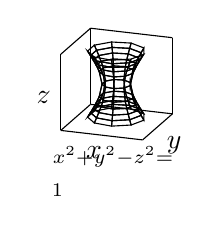
\begin{tikzpicture}
	\pgfplotsset{ticks=none}
    \begin{axis}[
            xmin=-3,xmax=3,
            ymin=-3,ymax=3,
            zmin=-2,zmax=2,
            xlabel={$x$},
            ylabel={$y$},
            zlabel={$z$},
            zlabel style={rotate=90},
            view={20}{20},
            width=3cm,
            height=3cm]
        % x^2+y^2-z^2=1
        \addplot3[mesh,black,domain=1:2,y domain=0:2*pi,samples=6,samples y=10]({x*cos(deg(y))},{x*sin(deg(y))},{sqrt(x^2-1)});
        \addplot3[mesh,black,domain=1:2,y domain=0:2*pi,samples=6,samples y=10]({x*cos(deg(y))},{x*sin(deg(y))},{-sqrt(x^2-1)});
    \end{axis}
    
    \node[text width=1.6cm] at (0.7,-0.4) {$\scriptstyle x^2+y^2-z^2=1$};
\end{tikzpicture}
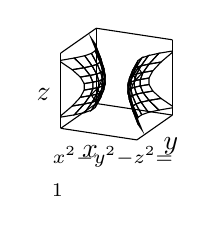
\begin{tikzpicture}
	\pgfplotsset{ticks=none}
    \begin{axis}[
            xmin=-3,xmax=3,
            ymin=-3,ymax=3,
            zmin=-2,zmax=2,
            xlabel={$x$},
            ylabel={$y$},
            zlabel={$z$},
            zlabel style={rotate=90},
            view={25}{20},
            width=3cm,
            height=3cm]
        % x^2-y^2-z^2=1
        \addplot3[mesh,black,domain=-1.2:1.2,y domain=-1.2:1.2,samples=8,samples y=8]({cosh(x)*cosh(y)},{cosh(x)*sinh(y)},{sinh(x)});
        \addplot3[mesh,black,domain=-1.2:1.2,y domain=-1.2:1.2,samples=8,samples y=8]({-cosh(x)*cosh(y)},{cosh(x)*sinh(y)},{sinh(x)});
        
    \end{axis}
    
    \node[text width=1.6cm] at (0.7,-0.4) {$\scriptstyle x^2-y^2-z^2=1$};
\end{tikzpicture}
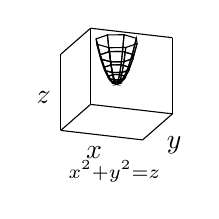
\begin{tikzpicture}
	\pgfplotsset{ticks=none}
    \begin{axis}[
            xmin=-3,xmax=3,
            ymin=-3,ymax=3,
            zmin=-2,zmax=2,
            xlabel={$x$},
            ylabel={$y$},
            zlabel={$z$},
            zlabel style={rotate=90},
            view={20}{20},
            width=3cm,
            height=3cm]
        \addplot3[mesh,black,domain=0:2*pi,y domain=0:1.5,samples=9,samples y=6]({y*cos(deg(x))},{y*sin(deg(x))},{y^2});
        
    \end{axis}
    
    \node[text width=1.2cm] at (0.7,-0.4) {$\scriptstyle x^2+y^2=z$};
\end{tikzpicture}
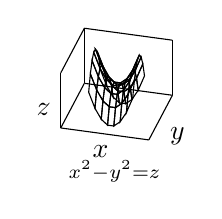
\begin{tikzpicture}
	\pgfplotsset{ticks=none}
    \begin{axis}[
            xmin=-3,xmax=3,
            ymin=-3,ymax=3,
            zmin=-2,zmax=2,
            xlabel={$x$},
            ylabel={$y$},
            zlabel={$z$},
            zlabel style={rotate=90},
            view={15}{40},
            width=3cm,
            height=3cm]
        \addplot3[mesh,black,domain=-1.5:1.5,y domain=-1.5:1.5,samples=8,samples y=8]({x},{y},{x^2-y^2});
        
    \end{axis}
    
    \node[text width=1.2cm] at (0.7,-0.4) {$\scriptstyle x^2-y^2=z$};
\end{tikzpicture}


\textbf{Sfera}: luogo dei punti dello spazio equidistanti da un punto fisso (centro). $x^2+y^2+z^2=r^2$

\textbf{Cono}: luogo di rette per un punto fisso (vertice, centro).

\textbf{Cilindro}: luogo di rette parallele.

Non tutti i coni/cilindri sono quadriche.

\textbf{Rotazioni}: ($z = 0$) $F(x, y)$ attorno $x$ diventa $F(x, \sqrt{y^2+z^2})$
$F(x,y,z)$ è di rotazione $\Leftrightarrow$ ha 2 autoval uguali, diversi da 0.

\begin{tabular}{cccl}
	\textbf{Equazione} & \textbf{Asse} & \textbf{Risultato} & \textbf{Nome} \\
	\hline
	$\frac{x^2}{a^2}+\frac{y^2}{b^2}=1$ & $x$ & $\frac{x^2}{a^2}+\frac{y^2+z^2}{b^2}=1$ & Ellis. di rot. \\
	$\frac{x^2}{a^2}-\frac{y^2}{b^2}=1$ & $x$ & $\frac{x^2}{a^2}-\frac{y^2+z^2}{b^2}=1$ & Iperb. ellit. \\
	$\frac{x^2}{a^2}-\frac{y^2}{b^2}=1$ & $y$ & $\frac{x^2+z^2}{a^2}-\frac{y^2}{b^2}=1$ & Iperb. iperb. \\
	$x^2=2py$ & $x$ & $x^2+z^2=2py$ & Parab. di rot.
\end{tabular}

\textbf{Fascio di quadriche}: $\lambda F(x, y, z) + \mu G(x, y, z) = 0$

\textbf{Forme canoniche}
\setlength{\tabcolsep}{0.2em}%
\begin{tabular}{llccc}
	\textbf{Equazione} & \textbf{Nome} & \textbf{Pnt.} & \textbf{Rig.} & \textbf{Cent.} \\
	\hline
	$\frac{x^2}{a^2} + \frac{y^2}{b^2} + \frac{z^2}{c^2} = 1$ & Ellissoide & E & No & Si \\
	$\frac{x^2}{a^2} + \frac{y^2}{b^2} - \frac{z^2}{c^2} = 1$ & Iperb. iperb. (1 falda) & I & Si & Si \\
	$\frac{x^2}{a^2} - \frac{y^2}{b^2} - \frac{z^2}{c^2} = 1$ & Iperb. ellitt. (2 falde) & E & No & Si \\
	$\frac{x^2}{a^2} + \frac{y^2}{b^2} = 2pz$ & Parab. ellitt. & E & No & No \\
	$\frac{x^2}{a^2} - \frac{y^2}{b^2} = 2pz$ & Parab. iperb. (sella) & I & Si & No \\
	 & Coni e cilindri & P & Si & \\
\end{tabular}

Quadrica $\cap$ piano tangente $=$ 1 retta (punto parabolico), 2 rette incidenti (punto iperbolico), 1 punto (punto ellittico). 

\textbf{Classificazione}
\begin{tabular}{ll}
	$I_1=\tr A = \lambda_1+\lambda_2+\lambda_3$ & $I_2=\lambda_1\lambda_2+\lambda_1\lambda_3+\lambda_2\lambda_3$ \\
	$I_3 = \det A$ & $I_4 = \det B$
\end{tabular}

{
\begin{threeparttable}
\setlength{\tabcolsep}{0.5em}%
\begin{tabular}{c|c|c|c|l|c|c|l}
	\boldmath$I_4$
	         & \boldmath$I_3$
	                 & \boldmath$I_2$
	                       & \boldmath$I_1$
	                               & \boldmath$\vec{x}^TA\vec{x}$\tnote{†}
	                                          & \boldmath$\rk A$
	                                              & \boldmath$\rk B$
	                                                     & \textbf{Quadrica} \\
	\hline
	+        & $\pm$ & $+$ & $\pm$ & def.     & 3 & 4    & Ellis. imm. \\
	+        & $\pm$ & $-$\tnote{‡} & $\mp$ & indef.   & 3 & 4    & Iperb. iperb. \\
	+        & 0     &     &       &          & 2 & 4    & Parab. iperb. \\
	\hline
	0        & $\pm$ & $+$ & $\pm$ & def.     & 3 & 3    & Cono imm. \\
	0        & $\pm$ & $-$ & $\mp$ & indef.   & 3 & 3    & Cono reale \\
	0        & 0     & $-$ &       & indef.    & 2 & 3    & Cilindro iperb. \\
	0        & 0     & $+$ &       & semi.   & 2 & 3    & Cilindro ellit. \\
	0        & 0     & 0   &       &          & 1 & 3    & Cilindro parab. \\
	0        & 0     &     &       &          & $\le 2$ & 2    & 2 piani distinti \\
	0        & 0     &     &       &          & 1 & 1    & 2 piani coincid. \\
	\hline
	$-$      & $\pm$ & $+$ & $\pm$ & def.     & 3 & 4    & Elliss. reale \\
	$-$      & $\pm$ & $-$\tnote{‡} & $\mp$ & indef.   & 3 & 4    & Iperb. ellit. \\
	$-$      & 0     &     &       &          & 2 & 4    & Parab. ellit. \\
\end{tabular}
\begin{tablenotes}
	\item[†] $\vec{x}^TA\vec{x}$ i termini di 2\textdegree\ grado, equivalente a valutare $I_1$ e $I_2$
	\item[‡] È suffciente che $I_1I_3 \le 0$ o $I_2 \le 0$
\end{tablenotes}
\end{threeparttable}
}


\section{Esercizi svolti}
\subsection{Diagonalizzazione di una matrice}
$
A = \left[
	\arraycolsep=2.0pt\def\arraystretch{1.0}
	\begin{array}{@{}ccc@{}}
		1 & 1 & 0 \\
		0 & k & 0\\
		0 & 0 & 2\\
	\end{array}
\right]
$
%\hspace{1cm}
\begin{tabular}{l}
	$p(\lambda) = \det(A-\lambda I) = (1-\lambda)(k-\lambda)(2-\lambda)$ \\
	$\lambda_1 = 1, \lambda_2 = 2, \lambda_3 = k$
\end{tabular}

Se $k\neq1$ e $k\neq2 \Rightarrow \lambda_1, \lambda_2, \lambda_3$ sono semplici e quindi regolari \\
$\quad\Rightarrow$ A è diagonalizzabile

% This is the "beauty" of LaTeX
Se $k = 1 \Rightarrow \lambda_2$ è semplice, studio $\lambda_1$: \\
$\quad V_1 = \ker(A-\lambda_1I) = \ker
\left(
	\left[
		\arraycolsep=2.0pt\def\arraystretch{1.0}
		\begin{array}{@{}ccc@{}}
			1 & 1 & 0 \\
			0 & 1 & 0\\
			0 & 0 & 2\\
		\end{array}
	\right] - I 
\right) = \ker
\left[
	\arraycolsep=2.0pt\def\arraystretch{1.0}
	\begin{array}{@{}ccc@{}}
		0 & 1 & 0 \\
		0 & 0 & 0\\
		0 & 0 & 1\\
	\end{array}
\right]$ \\
$\quad \Rightarrow \dim(V_1) = 1 \Rightarrow m_g \neq m_a$
$\ \Rightarrow \lambda_1$ non è regolare \\
$\quad \Rightarrow$ A non è diagonalizzabile


Se $k = 2 \Rightarrow \lambda_1$ è semplice, studio $\lambda_2$:\\
$\quad V_2 = \ker(A-\lambda_2I) = \ker
\left(
	\left[
		\arraycolsep=2.0pt\def\arraystretch{1.0}
		\begin{array}{@{}ccc@{}}
			1 & 1 & 0 \\
			0 & 2 & 0\\
			0 & 0 & 2\\
		\end{array}
	\right] - 2I 
\right) = \ker
\left[
	\arraycolsep=2.0pt\def\arraystretch{1.0}
	\begin{array}{@{}ccc@{}}
		-1 & 1 & 0 \\
		0 & 0 & 0\\
		0 & 0 & 0\\
	\end{array}
\right]$ \\
$\quad \Rightarrow \dim(V_2) = 2 \Rightarrow m_g = m_a$
$\ \Rightarrow \lambda_2$ è regolare \\
$\quad \Rightarrow$ A è diagonalizzabile

\subsection{Verifica similitudine}
\begin{tabular}{cc}
	$
	A_h = \left[
		\arraycolsep=2.0pt\def\arraystretch{1.0}
		\begin{array}{@{}ccc@{}}
			1   & 2 & 0 \\
			h+1 & 1 & 0 \\
			0   & 0 & 2 \\
		\end{array}
	\right]
	$ &
	$
	B = \left[
		\arraycolsep=2.0pt\def\arraystretch{1.0}
		\begin{array}{@{}ccc@{}}
			1 & 0 & 0 \\
			0 & 1 & 0 \\
			0 & 0 & 2 \\
		\end{array}
	\right]
	$
\end{tabular}

$p_A(\lambda) = (2-\lambda)(1+\sqrt{2(h+1)}-\lambda)(1-\sqrt{2(h+1)}-\lambda)$
$p_B(\lambda) = (2-\lambda)(1-\lambda)(1-\lambda)$

$A$ e $B$ devono avere gli stessi autovalori $\Rightarrow h = -1$

%Studio diagonalizzabilità di $A_{-1} =
%\left[
%	\arraycolsep=2.0pt\def\arraystretch{1.0}
%	\begin{array}{@{}ccc@{}}
%		1 & 2 & 0 \\
%		0 & 1 & 0 \\
%		0 & 0 & 2 \\
%	\end{array}
%\right]
%$
%
%$\lambda_1 = 2$ è semplice e quindi regolare. Studio $\lambda_2 = 1$ \\
%$V_1 = \ker 
%\left[
%	\arraycolsep=2.0pt\def\arraystretch{1.0}
%	\begin{array}{@{}ccc@{}}
%		0 & 2 & 0 \\
%		0 & 0 & 0 \\
%		0 & 0 & 1 \\
%	\end{array}
%\right]
%$
%$\Rightarrow \dim V_1 = 1 \neq m_a(1)$
%$\Rightarrow \lambda_2$ non è regolare.

$A_{-1}$ non è diagonalizzabile, non è simile a $B$ (diagonale).

\subsection{Conica a centro}
$\mathfrak{C}:\ 3x^2-2xy+3y^2-x-y-2=0$
$
A = \left[
	\arraycolsep=2.0pt\def\arraystretch{1.0}
	\begin{array}{@{}cc@{}}
		3  & -1 \\
		-1 & 3
	\end{array}
\right]
\
B = \left[
	\arraycolsep=2.0pt\def\arraystretch{1.0}
	\begin{array}{@{}ccc@{}}
		3  & -1 & -1/2 \\
		-1 & 3  & -1/2 \\
		-1/2  & -1/2 & -2 \\
	\end{array}
\right]
$
\begin{tabular}{l}
	$I_1 = \tr A = 6$ \\
	$I_2 = \det A = 8$ \\ 
	$I_3 = \det B = -18$
\end{tabular}

$I_2 \neq 0 \Rightarrow$ conica a centro. $I_1 I_3 < 0 \Rightarrow$ ellisse reale

Calcolo il centro che soddisfa $A \vec{v} = -\vec{b}$
$
\left[
	\arraycolsep=2.0pt\def\arraystretch{1.0}
	\begin{array}{@{}cc|c@{}}
		3  & -1 & 1/2 \\
		-1 & 3  & 1/2
	\end{array}
\right]
\rightarrow
\left[
	\arraycolsep=2.0pt\def\arraystretch{1.0}
	\begin{array}{@{}cc|c@{}}
		3  & -1   & 1/2 \\
		0  & 8/3  & 2/3 
	\end{array}
\right]
\Rightarrow
O'_{|\Base} =
\begin{bmatrix}
	1/4 \\[-0.3em]
	1/4 \\
\end{bmatrix}
$

Calcolo autospazi di $A$ (autovettori sono paralleli assi di $\mathfrak{C}$)
$p(\lambda) = \det(A-\lambda I) = (2-\lambda)(4-\lambda)$
$\ \Rightarrow \lambda_1 = 2, \lambda_2 = 4$
$V_2 = \Lin 
\begin{bmatrix}
	1 \\[-0.3em]
	1 \\
\end{bmatrix}
= \Lin
\begin{bmatrix}
	1/\sqrt{2} \\[-0.3em]
	1/\sqrt{2} \\
\end{bmatrix}
\quad
V_4 = \Lin 
\begin{bmatrix}
	-1 \\[-0.3em]
	1 \\
\end{bmatrix}
= \Lin
\begin{bmatrix}
	-1/\sqrt{2} \\[-0.3em]
	1/\sqrt{2} \\
\end{bmatrix}
$

Cambio di coordinate (nota che $Q \in SO(n)$):
$
\begin{bmatrix}
	x \\[-0.3em]
	y \\
\end{bmatrix}
= Q
\begin{bmatrix}
	x' \\[-0.3em]
	y' \\
\end{bmatrix}
+ O'_{|\Base} = 
\left[
	\arraycolsep=2.0pt\def\arraystretch{1.0}
	\begin{array}{@{}cc@{}}
		1/\sqrt{2} & -1/\sqrt{2} \\
		1/\sqrt{2} & 1/\sqrt{2}
	\end{array}
\right]
\begin{bmatrix}
	x' \\[-0.3em]
	y' \\
\end{bmatrix}
+
\begin{bmatrix}
	1/4 \\[-0.3em]
	1/4 \\
\end{bmatrix}
$

Essendo un ellisse: $\lambda_1x'^2 + \lambda_2y'^2 + t = 2x'^2 + 4y'^2 + t = 0$
$
B' = \left[
	\arraycolsep=2.0pt\def\arraystretch{1.0}
	\begin{array}{@{}ccc@{}}
		2 & 0 & 0 \\
		0 & 4 & 0 \\
		0 & 0 & t \\
	\end{array}
\right]
$
\begin{tabular}{l}
	$\Rightarrow I_3 = \det B' = 8t = \det B = -18$ \\
	$\Rightarrow t = -9/4$
\end{tabular}
$\Rightarrow \mathfrak{C'}:\ 2x'^2 + 4y'^2 -9/4 = 0$
$\Rightarrow \mathfrak{C'}:\ \frac{8}{9}x'^2 + \frac{16}{9}y'^2 = 1$

\subsection{Conica non a centro}
$\mathfrak{C}:\ x^2+4xy+4y^2-10\sqrt{5}x=0$
$
A = \left[
	\arraycolsep=2.0pt\def\arraystretch{1.0}
	\begin{array}{@{}cc@{}}
		1 & 2 \\
		2 & 4
	\end{array}
\right]
\
B = \left[
	\arraycolsep=2.0pt\def\arraystretch{1.0}
	\begin{array}{@{}ccc@{}}
		1          & 2 & -5\sqrt{5} \\
		2          & 4 & 0 \\
		-5\sqrt{5} & 0 & 0 \\
	\end{array}
\right]
$
\begin{tabular}{l}
	$I_1 = \tr A = 5$ \\
	$I_2 = \det A = 0$ \\ 
	$I_3 = \det B = -500$
\end{tabular}
$I_2 = 0 \Rightarrow$ conica non a centro. $I_3 \neq 0 \Rightarrow$ parabola

Calcolo autospazi di $A$ \\
$p(\lambda) = \det(A-\lambda I) = -\lambda(5-\lambda)$
$\ \Rightarrow \lambda_1 = 0, \lambda_2 = 5$
$V_0 = \Lin 
\begin{bmatrix}
	2 \\[-0.3em]
	-1 \\
\end{bmatrix}
= \Lin
\begin{bmatrix}
	2/\sqrt{5} \\[-0.3em]
	-1/\sqrt{5} \\
\end{bmatrix}
\quad
V_5 = \Lin 
\begin{bmatrix}
	1 \\[-0.3em]
	2 \\
\end{bmatrix}
= \Lin
\begin{bmatrix}
	1/\sqrt{5} \\[-0.3em]
	2/\sqrt{5} \\
\end{bmatrix}
$

Trovo la matrice U ortogonale che diagonalizza A e eseguo rotazione:
(nota che $U \in SO(2) \Rightarrow \det U = 1$ e $U$ ortonormale)
$
\begin{bmatrix}
	x \\[-0.3em]
	y \\
\end{bmatrix}
= U
\begin{bmatrix}
	\tilde{x} \\[-0.3em]
	\tilde{y} \\
\end{bmatrix}
=
\left[
	\arraycolsep=2.0pt\def\arraystretch{1.0}
	\begin{array}{@{}cc@{}}
		2/\sqrt{5} & 1/\sqrt{5} \\
		-1/\sqrt{5} & 2/\sqrt{5}
	\end{array}
\right]
\begin{bmatrix}
	\tilde{x} \\[-0.3em]
	\tilde{y} \\
\end{bmatrix}
$ \\
$
\Rightarrow \tilde{A} = U^TAU = \left[
	\arraycolsep=2.0pt\def\arraystretch{1.0}
	\begin{array}{@{}cc@{}}
		0 & 0 \\
		0 & 5
	\end{array}
\right]
,\quad
\tilde{\vec{b}} = U^T\vec{b} = \begin{bmatrix}
	-10 \\[-0.3em]
	-5 \\
\end{bmatrix}
,\quad
\tilde{c} = c
$ \\
$\Rightarrow \tilde{\mathfrak{C}}:\ 5\tilde{y}^2 - 20\tilde{x} - 10\tilde{y} = 0$ e completamento dei quadrati
$\Rightarrow \tilde{\mathfrak{C}}:\ 5(\tilde{y}-1)^2 - 20(\tilde{x}+1/4) = 0$ \\
$\Rightarrow 
\begin{bmatrix}
	x \\[-0.3em]
	y \\
\end{bmatrix}
= U
\begin{bmatrix}
	\tilde{x} \\[-0.3em]
	\tilde{y} \\
\end{bmatrix}
= U
\begin{bmatrix}
	x'-1/4 \\[-0.3em]
	y'+1 \\
\end{bmatrix}
= U 
\begin{bmatrix}
	x' \\[-0.3em]
	y' \\
\end{bmatrix}
+
\begin{bmatrix}
	1/(2\sqrt{5}) \\[-0.3em]
	9/(4\sqrt{5}) \\
\end{bmatrix}
$

$\Rightarrow \mathfrak{C}':\ 5y'^2 - 20x' = 0$
$\Rightarrow \mathfrak{C}':\ y'^2 - 4x' = 0$

\subsection{Trovare l'equazione di una conica}

Scrivere l'equazione della conica per $O=(0,0)$, $A=(1,1)$, $B=(1,-1)$ e tangente a $x=2$ in $C=(2,0)$.

\begin{tabular}{lll}
	$\overline{AB}: x = 1$ & $\overline{AC}: x+y-2=0$ & $\overline{BC}: x-y-2=0$
\end{tabular}

\textbf{Fascio}: $\lambda (x+y-2)(x-y-2) + \mu (x-1)(x-2) = 0$

Passaggio per $O$: $4\lambda+2\mu=0$, sostituendo: $x^2+y^2-2x=0$. Circonferenza di centro $(1, 0)$ e raggio $1$
\subsection{Riconoscere una quadrica}

$x^2 - 6xy - 4xz - 8y + 2z = 0$

\begin{tabularx}{\textwidth}{llX}
	$
		A = \left[
		\arraycolsep=2.0pt\def\arraystretch{1.0}
		\begin{array}{@{}ccc@{}}
			1 & -3 & -2 \\
			-3 & 0 & 0 \\
			-2 & 0 & 0 \\
		\end{array}
		\right]
	$ &
	$
		B = \left[
		\arraycolsep=2.0pt\def\arraystretch{1.0}
		\begin{array}{@{}cccc@{}}
			1 & -3 & -2 & 0 \\
			-3 & 0 & 0 & -4 \\
			-2 & 0 & 0 & 1 \\
			0 & -4 & 1 & 0
		\end{array}
		\right]
	$ &
	$\det A = 0$ \newline
	$\det B = 121$ \newline
\end{tabularx}

$\det B > 0$ e $\det A = 0 \implies$ paraboloide iperbolico

\subsection{Hamilton-Cayley}

Data $A = \left[
\arraycolsep=2.0pt\def\arraystretch{1.0}
\begin{array}{@{}ccc@{}}
1 & 2 \\
3 & 4 \\
\end{array}
\right]$ calcolare $A^4$.

$p(\lambda) = \lambda^2-5\lambda-2$, quindi $A^2=5A+2I$.

$A^4 = A^2A^2 = (5A+2I)(5A+2I) = 25A^2+20A+4I = 25(5A+2I)+20A+4I = 145A + 54I$
\subsection{Inversa di una funzione con Hamilton-Cayley}

Il polinomio caratteristico di $f$ è $p_f(\lambda) = -\lambda^3-4\lambda^2+5\lambda+3$.
Per Hamilton-Cayley $\Rightarrow p_f(A_f) = -A_f^3-4A_f^2+5A_f+3I = 0$
$\Rightarrow (3I)A_f^{-1} = (A_f^3+4A_f^2-5A_f)A_f^{-1}$
$\Rightarrow A_f^{-1} = (A_f^2+4A_f-5I)/3$
$\Rightarrow f^{-1} = (f^2+4f-5I)/3$


%%%%%%%%%%%%%%%%%%%%%%%%%%%%%%%%%%%%%%%%%%%%%%%%%%%%%%%%%%%%%%%%%%%%%%%%%%%%%%%%
\rule{0.3\linewidth}{0.25pt}
\scriptsize\\
\href{mailto:marco.donadoni@mail.polimi.it}{M. Donadoni}, \href{mailto:edoardo.morassutto@mail.polimi.it}{E. Morassutto},  Politecnico di Milano, A.A. 2016/17
\end{multicols}
\end{document}
